%%%%%%%%%%%%%%%%%%%%%%%%%%%%%%%%%%%%%%%%%%%%%%%%%%%%%%%%%%%%%%%%%%%%%%%%%%%%%%%%
%
% FILE: font_free_ocr.tex
%
% DESCRIPTION: LaTeX source file of ICDAR 2007 paper submission
%
% CVS:
% $Id: font_free_ocr.tex,v 1.5 2007-01-24 21:01:06 scottl Exp $
%
%%%%%%%%%%%%%%%%%%%%%%%%%%%%%%%%%%%%%%%%%%%%%%%%%%%%%%%%%%%%%%%%%%%%%%%%%%%%%%%%

% INITIALIZATION %
%%%%%%%%%%%%%%%%%%
\documentclass[times, 10pt,twocolumn]{article} 
\usepackage{latex8}
\usepackage{times}
\usepackage{graphicx}
\pagestyle{empty} %remove page numbers

% DOCUMENT START %
%%%%%%%%%%%%%%%%%%
\begin{document}

% TITLE %
%%%%%%%%%
\title{Shape-Free Character Identification for Optical Character Recognition}

% AUTHOUR INFO %
%%%%%%%%%%%%%%%%
\author{First Author\\
Addr 1\\
Addr 2\\
Addr 3\\
\and
Second Author\\
}

%@@the following is not to be included during the review process
%\author{Scott Leishman\\
%Department of Computer Science\\
%University of Toronto\\ 
%scottl@cs.toronto.edu\\
%\and
%Sam Roweis\\
%Department of Computer Science\\
%University of Toronto\\
%roweis@cs.toronto.edu\\
%}

\maketitle
\thispagestyle{empty}


% ABSTRACT %
%%%%%%%%%%%%
\begin{abstract}
@@to be written@@
\end{abstract}


% INTRODUCTION %
%%%%%%%%%%%%%%%%
\Section{Introduction}

Traditional approaches to optical character recognition (OCR) have typically
been reliant on font-specific shape information to convert bitmap
images of glyphs into corresponding sequences of ASCII or Unicode encoded
characters.  Some of the earliest systems were heavily restricted, only
able to recognize images that happened to closely match a template culled from
a database containing a handful of common typefaces in typical point
sizes.  Fortunately, modern systems have improved, and are now able to recognize
symbols from a much larger collection of varying fonts and character shapes.  
This has often been accomplished by using images or features of images from a 
wide array of font faces, styles, and sizes as labelled training data for 
character classifiers.  Even with this improved robustness, these systems 
still typically show degraded performance when presented with a document 
containing characters written in an unseen typeface or size.  
As electronic publishing becomes increasingly common (including the
ability for ordinary users to create their own custom fonts), the enormous
variety of fonts seen in printed and online documents continues to grow rapidly.
solely the domain of professional typographers, and as a result the number and 
variability of fonts seen in documents continues to rise.  
This creates an ongoing motivation to pursue font and shape
independent approaches to  optical character recognition.

Many previous attempts to ``font free'' character recognition share
the same general structure. Each page of ink is segmented into components
roughly corresponding to individual graphemes of the 
underlying document language. These components are clustered together in an 
unsupervised fashion based only on visual similarity.  For a language like 
English, the ideal result of this step would be a set of clusters such that
each one contains all occurrences of a particular 
character, digit, or punctuation symbol found in the document.
Of course, such exact clusterings are rarely achievable in practice, and 
trade-offs must be made between the final number of clusters and the 
consistency of the component members within a cluster.

In one of the earliest shape-free recognition approaches, Nagy et al. treated
the clustered sequence of components as the input cipher-text of a 
cryptogram\cite{nagy1987}.  Clusters were then assigned plain-text labels, 
with the assignment guided by the frequency of matches to words looked up in a 
small dictionary.

%@@@ Talk about Lee and Hull HMM approach too?  perhaps

Building on this, Ho and Nagy attempted to infer cluster labels using a series 
of simple statistical modules\cite{ho2000}.  Each module scores potential 
assignments using what they call a ``v/p ratio'', which counts the number of 
valid dictionary words that match the partially assigned word patterns that 
contain the cluster to be mapped.  In subsequent work, Ho and Nagy used 
several n-gram, frequency, and word-positional features to construct a 
classifier able to reliably determine whether an appropriately segmented 
cluster was an upper or lower case character, a digit, or a 
punctuation symbol\cite{ho2001}.

Recently, Huang et al. have used an entropy based approach to decode the
sequence of cluster identifiers representing individual words\cite{huang2006}.  
Confident mappings (those for which the distribution over character labels is 
sharply peaked at just a single label, given a dictionary of lookup words the 
same length as those that the cluster to be mapped appear in) are assigned 
first and used to narrow down the mappings for subsequent clusters.

In this paper we also pursue an approach to character recognition that 
makes no use of a priori character shape or font, instead relying entirely on 
contextual and statistical language cues to recognize character sequences.  
However, unlike several of the aforementioned attempts, we do not limit 
ourselves to the lowercase alphabetic characters of the English language. 
%@@briefly outline what we do differently@@


% CLUSTERING APPROACH %
%%%%%%%%%%%%%%%%%%%%%%%
\Section{Clustering Procedure}

Before attempts can be made to recognize the sequence of glyphs that 
constitute input document images, the appropriate elementary symbol regions 
must first be located, isolated, and clustered together.\footnote{The
discussion that follows assumes the document images given are not
already ``symbolically compressed''. Such a compression scheme will
store a single template image and the offset locations of each
appearance of that particular shape, even grouping together
those shapes that are slightly varied.  For input document images that
have been compressed in this way (via a JBIG2 compliant encoder 
for instance), a clustering procedure is often not necessary.}
After typical page image preprocessing steps like layout analysis, textual
region identification, deskewing, and noise removal are performed, the
connected components of ink on each page are identified and their bounding box
positions on the page are stored.  For each component, the nearest neighbouring
component in each of the four principal directions (top, bottom, left, and
right), as well as its pixel offset distance is also stored.  Individual lines
are then identified by following the chain of neighbouring components in
reading order.  The bounding box for a line is expanded as neighbour
component positions are read, and checks are made of neighbours in non-reading
order directions to determine if a line should be extended perpendicularly.

Since some symbols like {\em i, j, \'{e}, :, !} are made up of more than one
connected component, attempts are made to merge their constituent parts.  This
is accomplished by looking for separate components that belong to the same
line, are separated by a relatively small vertical distance (set manually), and
have one of the components completely overlapping the other horizontally.

Figure \ref{inimg_fig} displays a small region of input from a single document
page (top), for which the procedures described above have been run.

\begin{figure*}[ht]
  \centering
  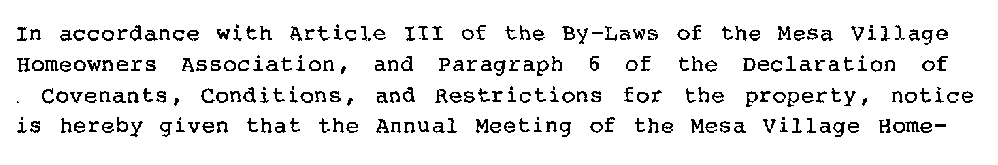
\includegraphics[scale=1]{figures/input_lines}
  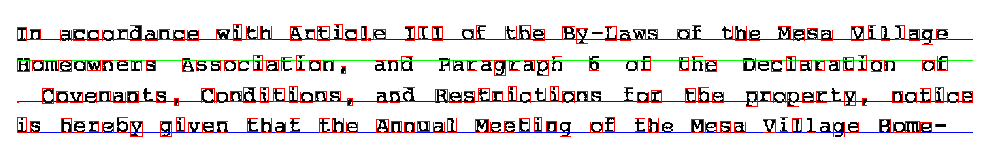
\includegraphics[scale=1]{figures/line_comps}
  \caption{Sample input image region and corresponding components, baselines,
           and x-heights found}
  \label{inimg_fig}
\end{figure*}

Each connected component image is initially assigned to its own cluster, then
clusters are merged in an agglomerative fashion.  First a simple Euclidean
distance measurement is taken between cluster centroid images, and those whose
value falls below a conservatively set threshold are merged together.  For near
noiseless documents with consistent symbol shapes, this has the effect of 
greatly reducing the number of clusters in a fairly efficient manner.

As Figure \ref{eucdist_fig} shows, one of the problems in calculating the 
Euclidean distance between two images is that each pixel difference is weighted 
equally regardless of where it occurs.  As a result two images of the same 
symbol that are either noisy or written in a slightly different font style or 
size could end up having a larger distance than that between images of 
different symbols.

\begin{figure}[ht]
  \centering
  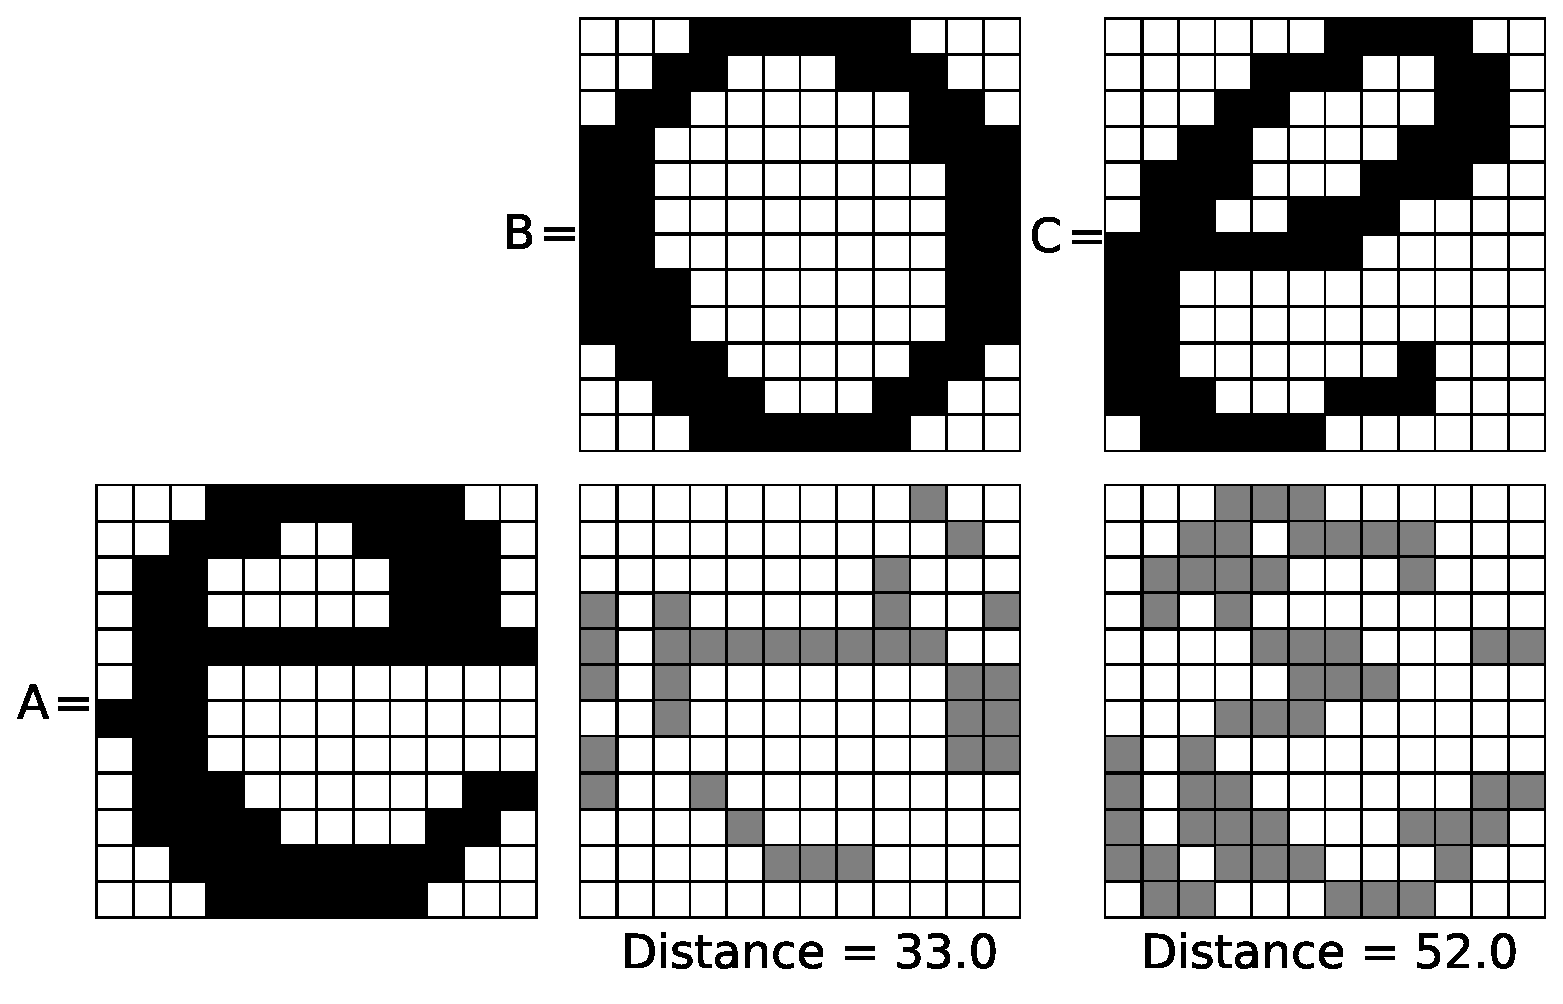
\includegraphics[scale=0.3]{figures/euc_dist_comparisons}
  \caption{Euclidean distance as calculated between a regular and italicized
  {\em e} versus the regular {\em e} and an {\em o} in the same font}
  \label{eucdist_fig}
\end{figure}

To attempt to combat the problems inherent in using Euclidean or other
unweighted distance metrics, the clusters are subsequently refined using the
Hausdorff distance\cite{rucklidge1996}.  The Hausdorff distance between two 
binary images $A$ and $B$ is typically defined as
\begin{eqnarray}
H(A,B) & = & \max(h(A,B), h(B,A))
\end{eqnarray}
where
\begin{eqnarray}
h(A,B) & = & \max_{a \in A} \min_{b \in B} || a - b ||
\end{eqnarray}
and $|| \cdot ||$ will be the $L_2$ (Euclidean) norm.

$h(A,B)$ can be interpreted as the directed Hausdorff distance from image $A$ to
image $B$, and means that for each foreground pixel in $A$ there is a foreground
pixel in $B$ that is no farther than $h(A,B)$ away, when the two images are 
laid over top one another.  Because the cluster average images may not be
binary, they are first thresholded so that they can be compared using this
metric.

To speed up processing, the Hausdorff distance is only calculated at the most
correlated position between each cluster average image.  This is found by
convolving the comparison image with a long image created by combining the
other cluster averages.  A Euclidean distance transform is then calculated on
this long image, with copies of the comparison image laid on top at the
appropriate positions, and the values at the 'on' pixels of the comparison 
image read off.  The maximum such value read on the pixels of each
comparison image defines the directed Hausdorff distance from the comparison 
image to that particular image.  The Euclidean distance transform is then
calculated on the comparison image, and a large tiled version is constructed
with appropriate padding to ensure that the previous long image can be laid on
top at the maximally correlated positions of each copy of the comparison image.
The underlying values at the 'on' pixels of each of the other images is then
read and the maximum taken to define the directed distance from the other
images to the comparison image.  Finally, the overall Hausdorff distance is
calculated by taking the maximum of these two directed distances for each
image.  Those that fall within a particular threshold ($\sqrt 2$ in our
experiments) are then clustered together.  Figure \ref{hausdist_fig}
shows this calculation between a few individual characters.

\begin{figure}[ht]
  \centering
  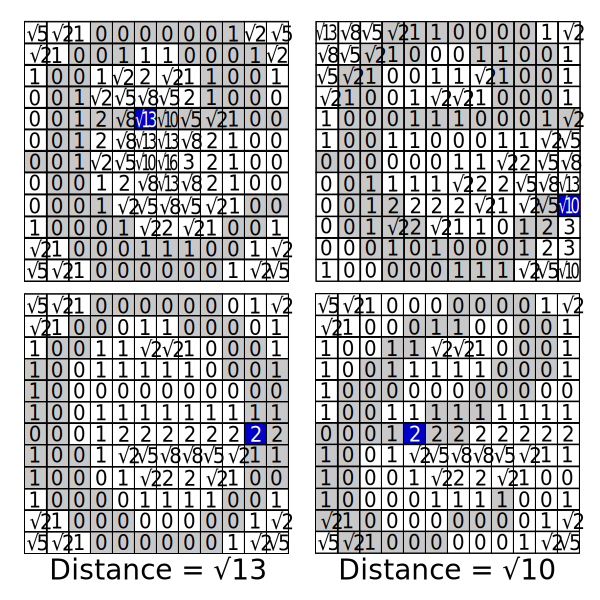
\includegraphics[scale=.5]{figures/haus_dist_comparisons}
  \caption{Hausdorff distance as calculated between a regular and italicized
  {\em e} versus the regular {\em e} and an {\em o} in the same font}
  \label{hausdist_fig}
\end{figure}

It should be noted that no attempts are made to normalize characters since the
Hausdorff distance combined with the averaging that takes place as components
are added to the clusters, can typically handle small deviations in font size.
While this may result in multiple clusters for the same symbol if font sizes
differ drastically, contextual procedures outlined in the following section
should still result in correct symbol recognition for all such clusters.

Depending on the font face, amount of kerning employed, and the quality of the
input document image, some glyphs may be broken into two or more pieces, or
they may end up touching one another resulting in a single component containing
multiple symbols.

To handle glyphs that have been broken apart, we attempt to recombine them by
examining the clusters that they belong to.  If components belonging to a
particular cluster tend to always lie adjacent to components in a second
cluster (and vice versa), and if the typical distance between these components
is relatively small, then they are merged.  In our experiments, those clusters
for which at least 85\% of the components share a neighbouring component in the
same second cluster, and are no farther than 3 pixels apart are merged.

Attempts are made to separate glyphs that have been smeared or so tightly
kerned that they are touching, by iteratively splitting the glyph near a
suspected boundary and trying to match each half with other cluster averages.
Provided both halves lie within a small Euclidean distance of their matching
clusters, the components of the original cluster are split at the appropriate
position, and added to their respective matching clusters.

This Hausdorff matching, cluster merging and splitting procedure is repeated
over those clusters that have had at least one change to their number of 
components at the previous iteration, until no further changes are seen.

With symbol clustering complete, a cluster is created to represent the blank
space between each word of documents written in alphabetic languages.
Inter-word space width is estimated in a simple fashion by counting the
frequency of component neighbour distances.  This distribution is typically
bi-modal with the first mode representing inter-character spacing, and a second
(often smaller) mode representing inter-word spacing.  The width assigned
is based on this second modal point, but is underestimated slightly to ensure no
actual inter-word spaces are missed.  New components are created representing
each of these spaces, and neighbours are updated appropriately.

Figure \ref{clavg_fig} shows the resulting cluster averages after this
procedure has been run on a single document taken from the Department of Energy
Sample 3 OCR dataset created by UNLV's ISRI group\cite{nartker2005}.

\begin{figure}[ht]
  \centering
  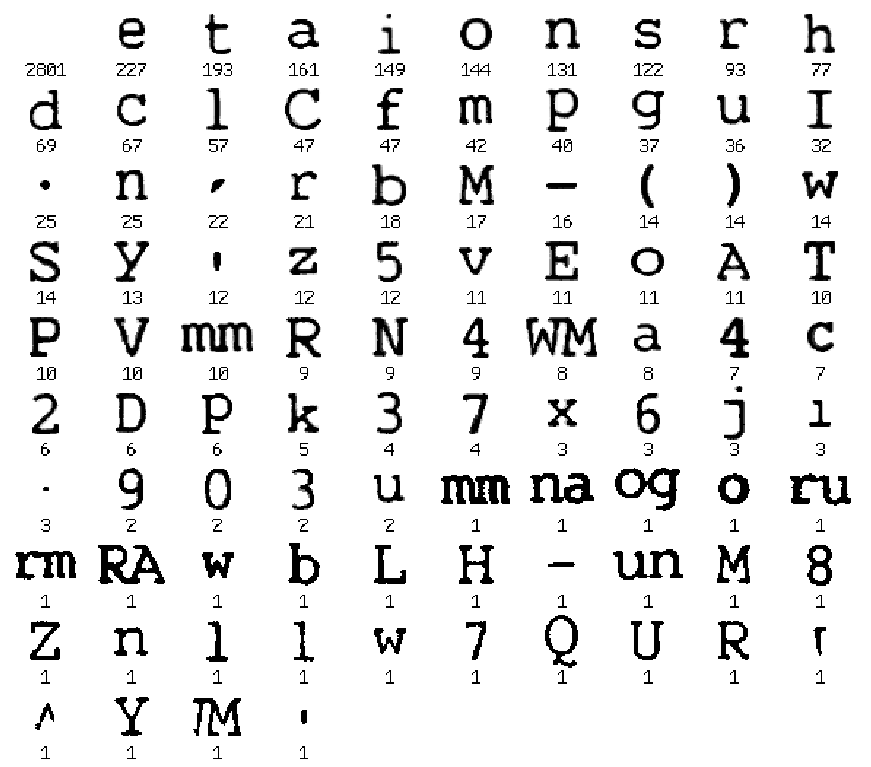
\includegraphics[scale=.5]{figures/cluster_averages}
  \caption{Typical cluster averages for a single document}
  \label{clavg_fig}
\end{figure}


% CONTEXTUAL RECOGNITION APPROACH %
%%%%%%%%%%%%%%%%%%%%%%%%%%%%%%%%%%%
\Section{Contextual Recognition}

With a reasonable clustering complete, the labels belonging to each cluster are
ready to be recognized.  Our contextual recognition approach has only been
tested on documents written in English, but should also be amenable to other
writing systems whose atomic symbols are roughly phonetic.  In our experiments
we have also assumed that we know in advance the script and language of the
input document, however previous research has shown it possible to infer this
automatically with relatively good accuracy\cite{sibun1994},\cite{hochberg1997}.

First a large text corpus is used to estimate overall word and symbol frequency,
as well as symbol positional frequency.  We take counts of the number of times
each symbol appears in each position of words up to a particular length.  As
a result of this, each symbol will then define a point in an $\frac{x
(x+1)}{2}$ dimensional ``positional'' feature space, where $x$ defines the
maximum word length to include (@@15@@ in our experiments).  We normalize each 
positional count by dividing by the total number of characters seen in the 
corpus.  @@paragraph may change since currently using a classifier approach@@

We repeat this process on the sequence of clustered components by gathering 
positional cluster frequency stats using the estimated components of the space 
symbol cluster to demarcate word boundaries.  By taking these counts over words
of length $x$ or less, we have that each cluster can be described as a point in
this ``positional'' feature space.

Determining which symbol each cluster belongs to is then a matter of first
ordering the output symbols based on their Euclidean distance to the cluster in
the ``positional'' feature space (starting with the closest).  For frequently
occurring symbols like lowercase vowels or common consonants, the closest
symbol is often the correct one, however for infrequently occurring symbols
whose feature vector could deviate wildly from that seen in a large corpus (due
to the domain and subject of the document for instance), this may not be the
case.

To determine the final symbol mapping chosen for each cluster, the ordering
determined by the positional distances are used.  Examining the clusters in
order starting with that the appeared most frequently in the document, each
symbol is tried in turn.  The current partially assigned mapping is applied to
the sequence of cluster identifiers in the document, and for each one in which
the current cluster appears, this symbol sequence is looked up for matches
against a large word corpus.  This ratio of the number of matches, to the total
number of cluster words in the input document is calculated, and provided that
it exceeds a particular threshold (75\% in our experiments), then that symbol
is permanently assigned to that particular cluster, and the mapping for the
next cluster is determined.

Initially, most of the dictionary words will match the cluster words since there
will only be a few clusters that have been assigned symbols.  However, these 
are also the most likely to be the correct mappings based purely on the
positional distances.  As more clusters are assigned symbols, it may become
impossible for a particular cluster to find a mapping that achieves a cluster
word to dictionary word ratio exceeding the desired threshold.  In such a case,
the symbol that achieves the largest such ratio is taken to be the correct
mapping.  @@discuss how ties will be broken?@@.  This process is repeated until
each of the clusters has been assigned a symbol.


% EXPERIMENTS %
%%%%%%%%%%%%%%%
\Section{Experiments}

To examine the validity of our proposed approach, we have run a series of tests
against the @@fine fax mode quality business letter dataset from the ISRI OCR
database\cite{nartker2005}.  Discuss the set used, no automatic zoning,
grouping pages belonging to the same document together@@

For our word lookup dictionary and our initial gathering of positional count
features, we made use of the first piece of the Reuters-21578 new
corpus\cite{lewis2004}.  After removing the tags and trailing ``Reuters''
byline from each article, we were left with 17601 unique words including many
proper nouns, digit strings, and other non-dictionary words.  This left us with
92 unique symbols, upon which to create positional counts from.  There were
744522 symbols in total.

After determining a final mapping from each cluster to a particular symbol, the
results where compared with the ground-truth text to determine recognition
accuracy.  Figure \ref{characc_fig} shows the resultant overall symbol
recognition accuracy as compared with the document size.  The average character
accuracy for the documents was found to be 53.19\% which is quite poor.

\begin{figure}[ht]
  \centering
  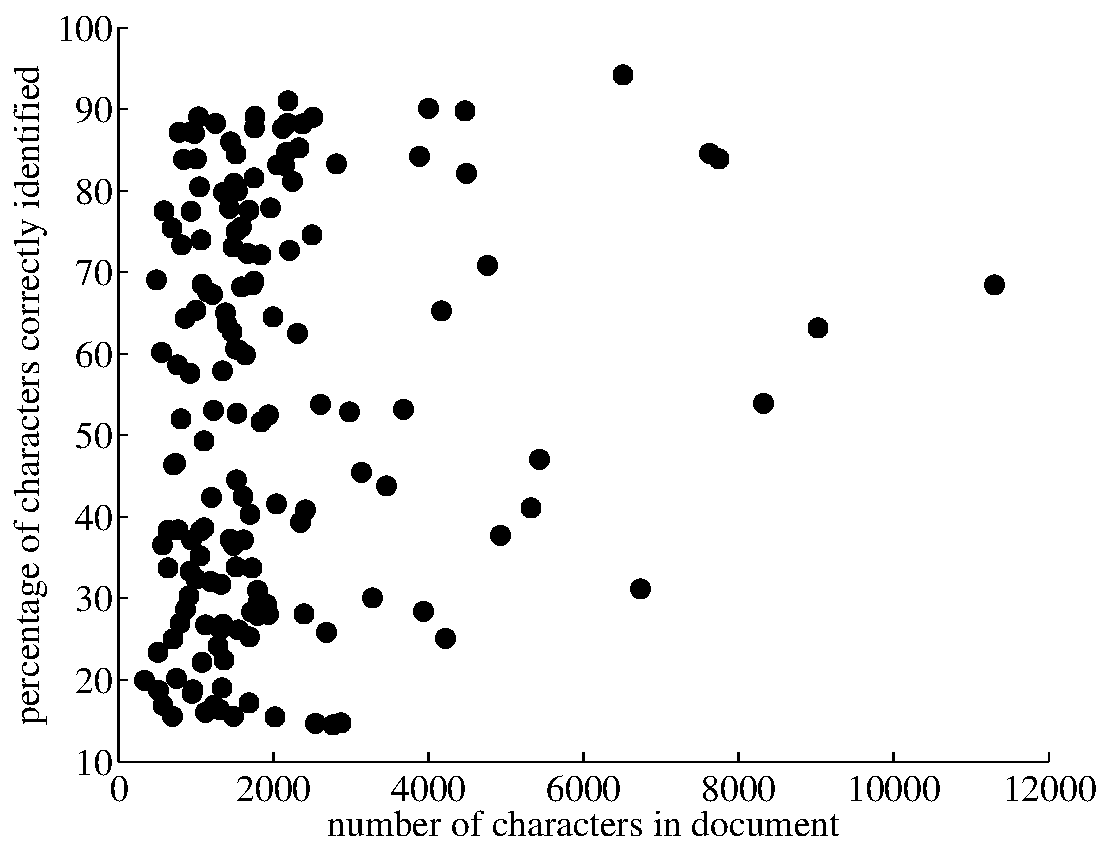
\includegraphics[scale=.4]{figures/character_accuracy}
  \caption{Scatter plot showing symbol recognition accuracy versus document
  size}
  \label{characc_fig}
\end{figure}

To determine how much an impact the clustering procedure has on performance,
the experiment above was repeated, but the ASCII ground truth symbols were
grouped together, representing a perfect segmentation and clustering.  Figure
\ref{gtcharacc_fig} shows the resultant recognition accuracy as a function of
document size.  The average character accuracy was found to be 80.17\% (with a
median accuracy of 88.77\%).  While this is much improved, it is still not on
par with typical recognition systems.  Most of the errors were not made on
lowercase characters, instead digits, punctuation symbols, and to a lesser
extent, upper case characters accounted for the majority of errors.

\begin{figure}[ht]
  \centering
  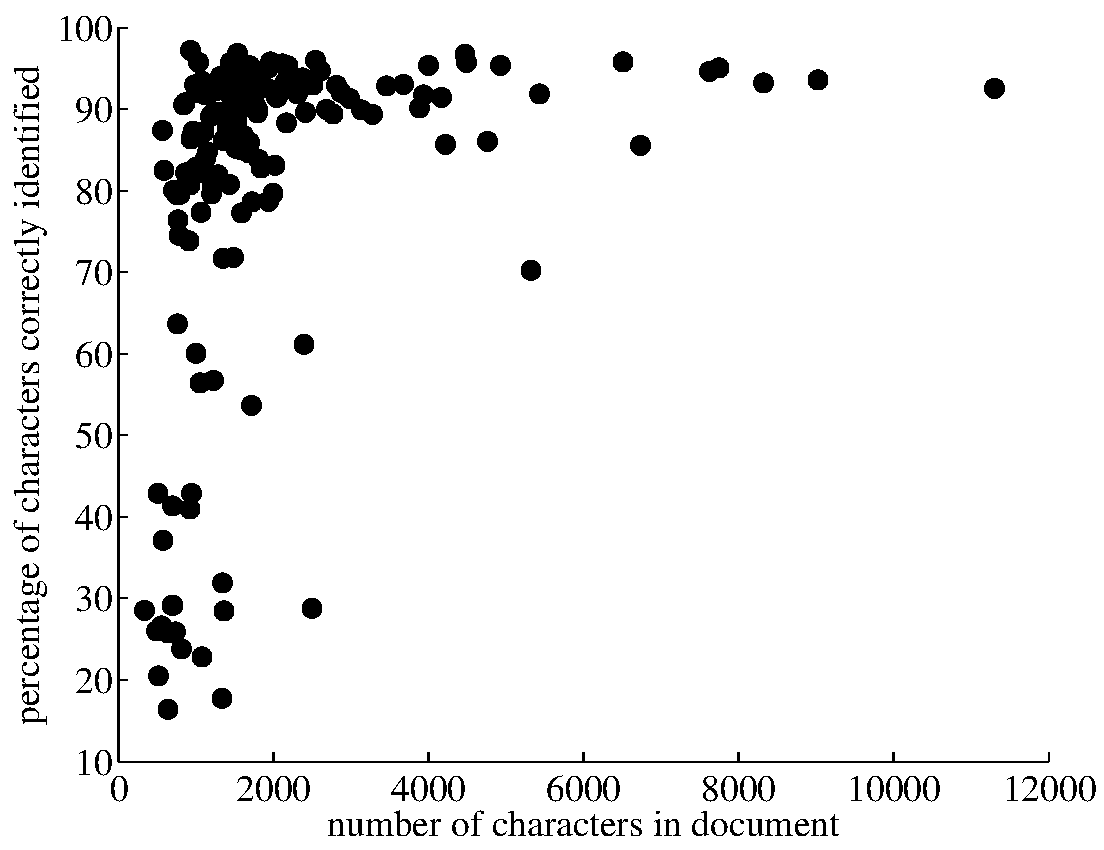
\includegraphics[scale=.4]{figures/gt_character_accuracy}
  \caption{Scatter plot showing ground-truth clustered symbol recognition 
  accuracy versus document size}
  \label{gtcharacc_fig}
\end{figure}

@@other experiments to be written@@


% CONCLUSIONS %
%%%%%%%%%%%%%%%
\Section{Conclusions}
@@to be written@@


% REFERENCES %
%%%%%%%%%%%%%%
\bibliographystyle{latex8}
\bibliography{font_free_ocr}

\end{document}
